\section{Introduction}\label{sec:intro}

Reinforcement learning (RL) has become a standard tool for synthesizing robotic controllers, with on-policy, weakly regularised algorithms such as Proximal Policy Optimisation (PPO) \citep{schulman2017proximal_PPO} serving as the de facto choice in many sim-to-real pipelines. Recent work has shown that carefully stabilised off-policy RL algorithms can match or outperform PPO in massively parallel simulators while also transferring to real legged robots, including humanoids and quadrupeds \citep{gallici2025simplifying_pqn, seo2025learning_fastsac, seo2025fasttd3, kim2026flashsac, rslrlsac2026bridging}. However, these evaluations primarily focus on nominal task performance, checking whether a policy can successfully perform the task under the conditions for which it was trained. In real-world deployment, policies must instead contend with changes in observations, environment properties, and system dynamics that are difficult to model exhaustively in simulation a priori. Robustness to such perturbations is therefore an important aspect of reliable sim-to-real transfer.

Regularisation provides a principled way to induce robustness. Regularised RL has long been successful in continuous-control and arcade-game benchmarks, where it can improve sample efficiency and stabilise optimisation \citep{dam2024unified_tree_search, haarnoja2018soft, ahmed_le_roux_2019_entropy_impact_pol_opt}. Beyond these practical benefits, a theoretical connection between regularised and robust RL suggests that regularisation can also provide implicit robustness to dynamics and task perturbations \citep{derman_twice_regularized, eysenbach2022maximum, pmlr-v130-husain21a_reg_pol_rew_rob, brekelmans2022_divergence_robustness}. This mechanism is complementary to Domain Randomisation (DR), which explicitly trains policies over a user-specified distribution of environment variations, such as changes to initial conditions or physical parameters \citep{eysenbach2022maximum, Mittal_Isaac_Lab_2025}. Whereas DR requires the practitioner to anticipate and specify the perturbations of interest, regularisation can induce robustness without explicitly enumerating them. This raises a natural empirical question: \textit{does the robustness induced by regularisation translate into more reliable real-world policy deployment?}

We study this question through the lens of the Soft MellowMax (SMM) operator. \citet{TGM_2025_jiralerspong} show that SMM induces a larger robust set than entropy regularisation, suggesting that it may provide stronger robustness to perturbations than the entropy regularisation used in methods such as Soft Actor-Critic (SAC) \citep{haarnoja2018soft}. However, SMM has primarily been studied in discrete state-action spaces, and extending it to continuous control is non-trivial because evaluating the operator requires integration over an intractable reference distribution. We address this challenge by introducing Soft MellowMax Actor-Critic (\ourMethod), an off-policy actor-critic algorithm that approximates the continuous SMM reference distribution with a dedicated, slowly updated reference policy. This provides a practical way to extend SMM-based regularisation to continuous control while maintaining stable actor-critic optimisation.


\begin{figure}
    \centering
    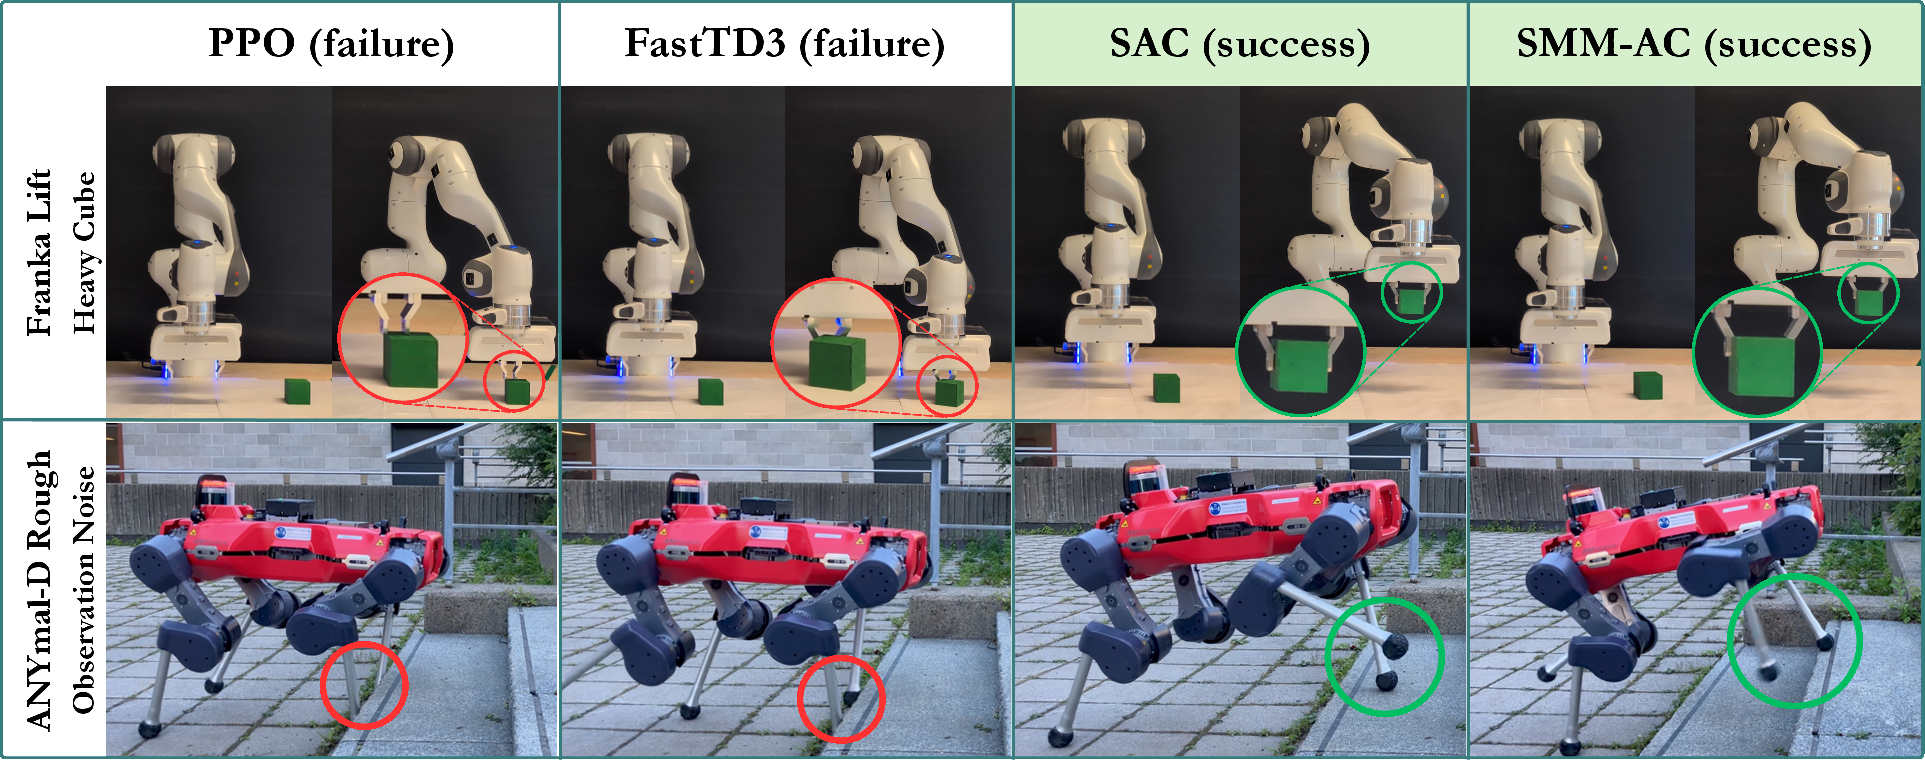
\includegraphics[width=\textwidth]{images/SMM-AC.pdf}
    \caption{\textbf{Overview of the Sim-to-Real Robustness Evaluation.} Top: Agents trained on the Franka Lift task in simulation are deployed with an object 2$\times$ heavier as those seen during training. The first frame shows the initial state, while the second shows the outcome, where the policy either successfully lifts the cube or fails to grasp it.
    Bottom: Agents trained on the ANYmal-D Rough task are deployed in the real world. Regularised algorithms have higher success rates in these sim-to-real settings.}
    \label{fig:intro_our_method_rocks}
\end{figure}

We evaluate \ourMethod alongside PPO, SAC, FastTD3, and other RL algorithms in simulation and on real-world robots, including a Franka arm and an ANYmal-D quadruped. In addition to nominal performance, we evaluate policies under deployment-time perturbations to observations, environment properties, and system dynamics. Across these experiments, regularised methods maintain higher performance under real-world perturbations, while \ourMethod achieves strong nominal performance and robustness across tasks. For example, when the mass of the object in the Franka cube-lifting task is doubled, PPO and FastTD3 fail to complete the task, whereas regularised methods successfully lift the cube. Similarly, regularised policies demonstrate greater robustness during rough-terrain locomotion on ANYmal-D (\autoref{fig:intro_our_method_rocks}). These results provide empirical evidence that the robustness associated with regularisation can translate into improved reliability during real-world deployment.

In this work,
\begin{itemize}[leftmargin=*, nosep]
\item we extend soft mellowmax to continuous state-action spaces and derive \textbf{Soft MellowMax Actor-Critic (\ourMethod)}, a practical off-policy actor-critic algorithm based on SAC (\autoref{sec:smm_ac});
\item we validate \ourMethod's performance in simulation on MuJoCo continuous-control benchmarks (\autoref{sec:mujoco});
\item we characterise the sim-to-real performance and real-world perturbation robustness of RL policies on Franka manipulation and ANYmal-D locomotion tasks, showing that regularised methods can maintain stronger performance under perturbations while achieving high nominal task performance (\autoref{sec:robotic}).
\end{itemize}
